\documentclass[a4paper, 12pt]{article}

\usepackage{amsfonts, amsmath, amsthm, enumitem, fancyhdr, graphicx, leftidx, physics}
\usepackage[explicit]{titlesec}

\title{\vspace{0cm} Quantum Information Theory}
\author{Erick Lin}

\pagestyle{fancy}
\renewcommand{\subsectionmark}[1]{}
\renewcommand{\sectionmark}[1]{\markright{\thesection.\ #1}}
\lhead{MATH/PHYS 4782}
\rhead{\rightmark}
% Show header on first page
\renewcommand{\thispagestyle}[1]{}

\titleformat{\section}{\normalfont\Large\bfseries}{}{0em}{\thesection.\ #1}

\numberwithin{equation}{section}
\numberwithin{figure}{section}

\newtheorem{theorem}{Theorem}[section]
\setcounter{theorem}{0}
\newtheorem{corollary}{Corollary}[theorem]
\newtheorem{lemma}[theorem]{Lemma}
\theoremstyle{definition}
\newtheorem{proposition}{Proposition}[section]
\setcounter{proposition}{0}
\newtheorem{definition}{Definition}[section]
\setcounter{definition}{0}
\newtheorem*{remark}{Remark}

\let\OLDthebibliography\thebibliography
\renewcommand\thebibliography[1]{
    \OLDthebibliography{#1}
    \setlength{\parskip}{0pt}
    \setlength{\itemsep}{0pt plus 0.3ex}
}

\newcommand{\prenote}{The first of these references is a comprehensive introductory textbook on quantum computation and quantum information, whose chapters 11 and 12, ``Entropy and information'' and ``Quantum information theory'', proved to be beneficial for this report. In learning the background knowledge and gathering materials, the author found Peter Shor's expositional article on the state of quantum information theory to be useful as well. However, this report is most deeply indebted to John Preskill's Caltech lectures on quantum information theory, from which it borrows most of the content and presentation of the subject.}

\makeatletter
\renewenvironment{thebibliography}[1]
     {\section*{\refname}%
      \@mkboth{\MakeUppercase\refname}{\MakeUppercase\refname}%
      \prenote
      \list{\@biblabel{\@arabic\c@enumiv}}%
           {\settowidth\labelwidth{\@biblabel{#1}}%
            \leftmargin\labelwidth
            \advance\leftmargin\labelsep
            \@openbib@code
            \usecounter{enumiv}%
            \let\p@enumiv\@empty
            \renewcommand\theenumiv{\@arabic\c@enumiv}}%
      \sloppy
      \clubpenalty4000
      \@clubpenalty \clubpenalty
      \widowpenalty4000%
      \sfcode`\.\@m}
     {\def\@noitemerr
       {\@latex@warning{Empty `thebibliography' environment}}%
      \endlist}
\makeatother

\allowdisplaybreaks

\begin{document}

    \maketitle

    \section{Introduction}
    In the words of Claude Shannon, the author of the famous 1948 paper, information theory concerns the fundamental problem of ``reproducing at one point \dots a message selected at another point''. Shannon solved the problems of
    \begin{enumerate}
        \item
            How much a message can be compressed, or the redundancy of the information (the source/noiseless coding theorem).

        \item
            At what rate information can be communicated reliably over a noisy channel, or the amount of redundancy that should be introduced to safeguard against errors (the noisy channel coding theorem).
    \end{enumerate}
    Quantum information theory is the branch of information theory in which the message or the method of reproduction involve quantum effects. Although the study of these effects was marginalized until fairly recently, one of the central issues which has no classical analog is that nonorthogonal pure quantum states cannot be perfectly distinguished. Broadly, quantum information theory concerns the topics of
    \begin{enumerate}
        \item
            Transmission of classical information over quantum channels,

        \item
            The tradeoff between acquisition of information about and disturbance of a quantum state,

        \item
            Quantifying quantum entanglement,

        \item
            Transmission of quantum information over quantum channels,
    \end{enumerate}
    which all rely on the concept of von Neumann entropy. Understanding and applying Von Neumann entropy, which can be considered as the quantum analog of Shannon entropy, is often a central tenet of much of quantum information theory. First, it is beneficial to define Shannon entropy from classical information theory and develop its relation to von Neumann entropy, before laying the groundwork for further topics in quantum information theory.

    \section{Shannon Entropy \label{sec:shannon}}
    Every property of a physical system can be associated with a random variable $X$ before its value is observed. The amount of uncertainty $X$, which can also be characterized as the amount of information gained when the value of $X$ is obtained, is quantified by \textit{Shannon entropy}, which we define as
    \begin{align}
        H(X) \equiv H(p_1, \cdots, p_n) \equiv -\sum_x p_x \log_2 p_x
    \end{align}
    where $p_1, \cdots, p_n$ comprise the probability distribution of the possible values $X$ can take. For the remainder of the text, we will use the symbol ``$\log$'' to abbreviate ``$\log_2$.'' By convention, if $p_x = 0$, then the corresponding event is not included in the entropy calculation because $\lim_{x \to 0} x \log x = 0$.
    Another perspective on entropy is that it quantifies the minimal amount of resources required to store information. Shannon's original paper introduced the \textit{source/noiseless coding theorem}, which states that $n H(X) + o(n)$ is the number of bits required to encode all the information of the $n$ outputs of a random variable $X$. This has applications in data compression, where the goal is to minimize the amount of space required to store data. Intuitively, the more frequently a value results from a random variable, the fewer number of bits we want to use encode that value, so that the total number of bits used is less than if the values were all equally weighted in the number of bits. \par
    For the special case of Bernoulli random variables, the Shannon entropy is called the \textit{binary entropy}, defined as
    \begin{align}
        H_{\text{bin}}(p) \equiv -p \log p - (1 - p) \log(1 - p)
    \end{align}
    where $p$ is the probability of one of the two outcomes. Note that $H(p) = H(1 - p)$ and $H(p)$ is maximized at $p = 1/2$. \par
    When two or more probability distributions are mixed together, additional information is gained from obtaining a value as compared to the average of the information gained from obtaining the same value from each probability distribution alone. If we have two Bernoulli random variables, one with parameter $p_1$ and the other with parameter $p_2$, and the probability of a result coming from the first random variable is $q$, then the previous statement tells us that
    \begin{align}
        H_{\text{bin}}(qp_1 + (1 - q)p_2) \geq qH_{\text{bin}}(p_1) + (1 - q)H_{\text{bin}}(p_2).
    \end{align}
    This is actually the definition of a \textit{concave function} if $H$ is the function and $p_1$ and $p_2$ are the inputs \cite{qc}. \par
    The \textit{relative entropy} of the probability distribution $p(x)$ to the distribution $q(x)$ is a distance measure between the two probability distributions over the same index set $x$, and is defined as
    \begin{align}
        H(p(x)||q(x)) \equiv \sum_x p(x) \log\frac{p(x)}{q(x)} = H(X) - \sum_x p(x) \log q(x),
    \end{align}
    where, in addition to the previous convention, $-p(x) \log 0 \equiv +\infty$ if $p(x) > 0$. \par
    The \textit{joint entropy} $H(X, Y)$ of two random variables $X$ and $Y$ is the entropy of the joint distribution of $X$ and $Y$, and if $\{ X_i \}$ denotes the set of possible values of $X$, then the \textit{conditional entropy} is given by
    \begin{align}
        H(Y | X) \equiv \sum_i H(Y | X = X_i) \mathbb{P}(X = X_i).
    \end{align}
    The \textit{mutual information} $I$ is given by
    \begin{align}
        I(X; Y) &\equiv H(Y) - H(Y | X) \label{sec:mutual1} \\
        &= H(X) - H(X | Y) \\
        &= H(X) + H(Y) - H(X, Y), \label{sec:mutual2},
    \end{align}
    which is symmetric and nonnegative (the inequalities $H(X) \geq H(X|Y) \geq 0$ can be proved using the convexity of the log function). The mutual information quantifies the correlation of two messages given by the random variables $X$ and $Y$, and can be thought of as the amount learned about one random variable when the value of the other becomes known. \par
    This leads up to the second of Shannon's main theorems, the \textit{noisy channel coding} theorem, which states that if $N$ is a noisy channel and $C$ is the \textit{channel capacity} given by
    \begin{align}
        C \equiv \max_{p(X)} I(X; N(X))
    \end{align}
    where $p(X)$ is the set of probability distributions on inputs $X$ to the channel and $N(X)$ is the corresponding output of the channel, then $n$ uses of $N$ can reliably communicate $Cn - o(n)$ bits with high probability. \par
    The proofs will be described in later sections, where they will play an important role and parallel many topics in the quantum version of information theory.

    \iffalse
    \section{Quantum Mechanics Background}
    In an $n$-dimensional quantum system $\mathcal{H}$, a \textit{von Neumann measurement} corresponds to a set of orthogonal subspaces $S_1, S_2, \cdots, S_k$ of $\mathcal{H}$ such that the $S_i$ span $\mathcal{H}$; in other words, $\sum_i \text{dim} S_i = n$. Let $P_i$ be the projection matrix onto each subspace $S_i$. Then given a density matrix $\rho$, the von Neumann measurement corresponding to the set $\{ S_i \}$ projects $\rho$ into the subspace $S_i$ with probability $\text{Tr}(P_i \rho)$. Following the projection, the state becomes the renormalized form of $P_i \rho P_i$. In the case that the $S_i$ are all one-dimensional so that $S_i = w_i w_i^\dagger$ and $\{ w_i \}$ forms an orthogonal basis of $\mathcal{H}$, the projection of a vector $v$ is $w_i$ with probability $|w_i^\dagger v|^2$ and the projection of a density matrix $\rho$ is $w_i$ with probability $w_i^\dagger \rho w_i$.
    \fi

    \section{Von Neumann Entropy}
    Now consider a system of $n$ qubits where each is in the state $\ket{0}$ or $\ket{1}$ with probability $\frac{1}{2}$. Any two of these states are completely distinguishable, so there are $2^n$ possible states, and the entropy is $n$ bits. However, if each each qubit is instead in the state $\ket{0}$ or $\frac{\ket{0} + \ket{1}}{\sqrt{2}}$ with equal probability, then the states are no longer completely distinguishable. Because there are less than $2^n$ possible states, the entropy is less than $n$ bits. \par
    Entropy in this sense is analogous to the concept of entropy from the field of thermodynamics, which relates work extracted from some physical system. Von Neumann used this approach to deduce the \textit{von Neumann entropy} of a quantum system with density matrix $\rho$, which is defined as
    \begin{align}
        S(\rho) \equiv -\text{Tr}(\rho \log\rho).
    \end{align}
    The above definition is justified from the fact that a density matrix$\rho$ is positive semidefinite. If $\rho$ is diagonalized in an orthonormal basis $\{ \ket{i} \}$so that it has eigenvalues $\lambda_i$, then $-\rho \log\rho$ is also diagonal with eigenvalues $-\lambda_i \log\lambda_i$. As a result
    \begin{align}
        S(\rho) = H(A)
    \end{align}
    where $H(A)$ is the Shannon entropy of the ensemble $A = \{ a, \lambda_a \}$. This means that the von Neumann entropy of a density matrix is the Shannon entropy of its eigenvalues. \par
    In the case where the signal space consists of mutually orthogonal pure states, the quantum source reduces to the classical case where the signal states can be perfectly distinguished, and $S(\rho) = H(X)$. For a quantum source that is not mutually commuting, we will show that the von Neumann entropy quantifies both the
    \begin{enumerate}
        \item
            quantum information content, or the minimum number of qubits per letter required to reliably encode the information, and the
        \item
            classical information content, or the maximum amount of information per letter in bits that can be learned about the preparation through measurement,
    \end{enumerate}
    per element of the ensemble. In addition, we will also find that von Neumann information plays a role in quantifying the entanglement of a bipartite pure state. A number of mathematical properties of von Neumann entropy are enumerated as follows.
    \begin{enumerate}[label=\textbf{(\arabic*)}]
        \item
            \textbf{Purity}. A pure state $\rho = \ket{\varphi} \bra{\varphi}$ has $S(\rho) = 0$.

        \item
            \textbf{Invariance}. The entropy is unchanged by a unitary change of basis:
            \begin{align}
                S \left( U \rho U^{-1} \right) = S(\rho),
            \end{align}
            since $S(\rho)$ depends only on the eigenvalues of $\rho$.

        \item
            \textbf{Maximum}. If $\rho$ has $D$ nonvanishing eigenvalues, then
            \begin{align}
                S(\rho) \leq \log D,
            \end{align}
            with equality if and only if all the nonzero eigenvalues are equal. This implies that the entropy is maximized when the quantum state is chosen randomly.

        \item
            \textbf{Concavity}. For $\lambda_1, \lambda_2, \cdots, \lambda_n \geq 0$ and $\lambda_1 + \lambda_2 + \cdots + \lambda_n = 1$,
            \begin{align}
                S(\lambda_1 \rho_1 + \cdots + \lambda_n \rho_n) \geq \lambda_1 S(\rho_1) + \cdots + \lambda_n S(\rho_n).
            \end{align}
            In other words, the von Neumann entropy is larger the more ignorant we are about how the state was prepared. The proof comes from the convexity of the log function.

        \item
            \textbf{Entropy of measurement}. Suppose that, in a state $\rho$, we measure the observable
            \begin{align}
                A = \sum_y \ket{a_y} a_y \bra{a_y}
            \end{align}
            so that the outcome $a_y$ occurs with probability
            \begin{align}
                p(a_y) = \matrixel{a_y}{\rho}{a_y}.
            \end{align}
            Then the Shannon entropy of the ensemble of measurement outcomes $Y = \{ a_y, p(a_y) \}$ satisfies
            \begin{align}
                H(Y) \geq S(\rho),
            \end{align}
            with equality if and only if $A$ and $\rho$ commute. Mathematically, $S(\rho)$ increases when all off-diagonal matrix elements of $\rho$ are replaced by $0$; physically, the randomness of the measurement outcome is minimized if the observable chosen for measurement commutes with the density matrix.

        \item
            \textbf{Entropy of preparation}. If a pure state is drawn randomly from the ensemble $\{ \ket{\varphi_x}, p_x \}$ so that the full density matrix is
            \begin{align}
                \rho = \sum_x p_x \ket{\varphi_x} \bra{\varphi_x},
            \end{align}
            then
            \begin{align}
                H(X) \geq S(\rho),
            \end{align}
            with equality if and only if the signal states $\ket{\varphi_x}$ are mutually orthogonal. In other words, distinguishability is lost when nonorthogonal pure states are mixed together.

        \item
            \textbf{Subadditivity}. For a bipartite system $AB$ in the state $\rho_{AB}$,
            \begin{align}
                S(\rho_{AB}) \leq S(\rho_A) + S(\rho_B)
            \end{align}
            where $\rho_A = \text{tr}_B \rho_{AB}$ and $\rho_B = \text{tr}_A \rho_{AB}$, with equality, or \textit{additivity}, when $\rho_{AB} = \rho_A \otimes \rho_B$ (the systems are uncorrelated). This property is also true for Shannon entropy since the mutual information for any two random variables is nonnegative.

        \item
            \textbf{Strong subadditivity}. For any state $\rho_\text{ABC}$ of a tripartite system,
            \begin{align}
                S(\rho_\text{ABC}) + S(\rho_B) \leq S(\rho_\text{AB}) + S(\rho_\text{BC}).
            \end{align}
            This property reduces to subadditivity in the case that $B$ is one-dimensional, and also holds for Shannon entropy. If $AB$ and $BC$ are regarded as two overlapping subsystems, then it can be thought that the entropy of their union $ABC$ added to the entropy of their intersection $B$ is at most the sum of the entropies of the subsystems.

        \item
            \textbf{Triangle (Araki-Lieb) inequality}. For a bipartite system,
            \begin{align}
                S(\rho_\text{AB}) \geq |S(\rho_A) - S(\rho_B)|.
            \end{align}
            The analogous property of Shannon entropy is
            \begin{align}
                H(X, Y) \geq H(X), H(Y)
            \end{align}
            or
            \begin{align}
                H(X | Y), H(Y | X) \geq 0.
            \end{align}
            In the classical case, the Shannon entropy of a bipartite system exceeds the Shannon entropy of either subsystem, which implies that the whole state contains more information than its parts. In the case of a bipartite pure quantum state, we have $S(\rho_A) = S(\rho_B)$ (nonzero if the state is entangled) and $S(\rho_\text{AB}) = 0$. Because information is encoded in nonlocal quantum correlations, it is not possible to deduce how the state was prepared by observing the subsystems separately.
    \end{enumerate}

    \section{Ties to Thermodynamics}
    The mathematical properties of the von Neumann entropy holds a number of implications for thermodynamics which can now be discussed. Two distinct but related approaches to quantum statistical physics are to consider the evolution of a closed quantum system while performing \textit{coarse graining} (reducing the number of degrees of freedom) to define thermodynamic variables, and to consider the evolution of an open system without keeping track of its environment. \par
    For an open system, the subadditivity of the von Neumann entropy is essential. If a system $A$ and an environment $E$ are initially uncorrelated with one another,
    \begin{align}
        \rho_{AE} = \rho_A \otimes \rho_Ek,
    \end{align}
    then the entropy is additive:
    \begin{align}
        S(\rho_{AE}) = S(\rho_A) + S(\rho_E).
    \end{align}
    The evolution of the open system is described by a unitary operator $U_\text{AE}$ that acts on the combined system:
    \begin{align}
        \rho_\text{AE} \to \rho_\text{AE}' = U_\text{AE} \rho_\text{AE} U_\text{AE}^{-1},
    \end{align}
    while
    \begin{align}
        S(\rho_\text{AE}') = S(\rho_\text{AE})
    \end{align}
    since $S$ is preserved under unitary transformations. Applying subadditivity to the state $\rho_\text{AE}'$,
    \begin{align}
        S(\rho_A) + S(\rho_E) = S(\rho_\text{AE}') \leq S(\rho_A') + S(\rho_E'),
    \end{align}
    with equality if and only if $A$ and $E$ remain correlated. The sum of the entropy of the system and the entropy of the environment (the entropy of the universe) cannot decrease, which is one form of the second law of thermodynamics. \par
    Under the \textit{Markovian approximation}, if the time resolution is course enough, then the system and environment begin in an uncorrelated state at each instant in time, and the entropy of the universe increases monotically, asymptotically approaching a maximum. \par
    The assumption from statistical physics is that the state and environment are in the configuration that maximizes $S(\rho_A) + S(\rho_E)$, which means that all possible states are equally likely. \par
    Microscopically, information initially encoded in the system is lost as it becomes encoded in quantum entanglement between the system and environment, which explains thermodynamic irreversibility. \par
    The arguments above can be applied to any large closed system that is divided up into a small part and its environment, in a form of coarse graining. The small part acts as an open system, which is why microcanonical and canonical ensembles in statistical mechanics give the same results for large systems.

    \section{Source Coding and Data Compression}
    While the original definition of entropy arose from the study of thermodynamics, and we learned that Shannon entropy holds a precise interpretation in classical information theory, we will find that von Neumann plays a parallel role in quantum information theory. \par
    Note that we use fidelity as a measure of indistinguishability -- the probability of success on a test that determines whether the output is the same as the input. Recall that given the original signal (which is a vector)
    \begin{align}
        u = \bigotimes_{i = 1}^n v_i,
    \end{align}
    where the $v_i$ are pure states, the fidelity between the signal $u$ and the output $\rho$ (a density matrix on $n$ qubits) is defined as
    \begin{align}
        F = u^\dagger \rho u.
    \end{align}
    In the case that the output is a pure state $v$, $F = u^\dagger vv^\dagger u = |u^\dagger v|^2$. \par
    Now, consider a long message consisting of $n$ letters, where each letter is chosen at random from the ensemble of pure states
    \begin{align}
        \{ \ket{\varphi_x}, p_x \}
    \end{align}
    and the $\ket{\varphi_x}$ are not necessarily mutually orthogonal (one physical example of $\ket{\varphi_x}$ might be the polarization state of a photon). Then each letter is described by the density matrix
    \begin{align}
        \rho = \sum_x p_x \dyad{\varphi_x}{\varphi_x}
    \end{align}
    and the message has the density matrix given by the tensor product $\rho^n$. \par
    An interesting problem lies in finding the \textit{quantum code} that compresses the message into the smallest possible Hilbert space while preserving the fidelity of the message. One immediate application of this would be finding the minimal possible usage of space in a quantum memory device, such as a hypothetical hard disk of a quantum computer, given that we know the statistical properties (which can be given by $\rho$) of recorded data on the disk. \par
    The solution, known as the \textit{Schumacher compression}, in the limit as $n \to \infty$ is given by compression to a Hilbert space $\mathcal{H}$ with
    \begin{align}
        \log(\dim \mathcal{H}) = n S(\rho);
    \end{align}
    thus, paralleling the noiseless coding theorem, the von Neumann entropy gives the exact number of qubits of quantum information carried per letter in the message. This means that if each letter is a photon polarization state, then the message may be compressed to $m = n S(\rho)$ photons. It is always compressed to a smaller size unless $\rho = \frac{1}{2} I$ (where $I$ is the identity matrix), which describes random qubits. Recall that random bits cannot be compressed according to the noiseless coding theorem as well. \par
    \iffalse
    For an example demonstrating Schumacher's data compression protocol, suppose that letters are drawn from the ensemble
    \begin{align}
        &\ket{0} = \left( \begin{array}{c}
            1 \\
            0
        \end{array} \right), \quad p = \frac{1}{2} \\
        &\frac{\ket{0} + \ket{1}}{\sqrt{2}} = \left( \begin{array}{c}
            1/\sqrt{2} \\
            1/\sqrt{2}
        \end{array} \right), \quad p = \frac{1}{2}
    \end{align}
    which gives, for each letter, the density matrix
    \begin{align}
        \rho = \frac{1}{2} \ket{0} \frac{\bra{0} + \bra{1}}{\sqrt{2}}
    \end{align}
    \fi
    To restate, given a memoryless quantum source that at each time step emits the pure state $v_i$ with probability $p_i$, the goal is to minimize the bits used to encode the signal in a way that the original state can still be reconstructed, even though it cannot be perfectly transmitted. Furthermore, quantum information theory differs from the classical in that the original state cannot be reconstructed perfectly most of the time, because the state to be reconstructed is nearly indistinguishable from the original state almost all the time. \par

    \subsection{Proofs of the Classical and Quantum Source Coding Theorems}
    The proof of the classical source coding theorem, introduced in Section \ref{sec:shannon}, is as follows. Suppose a memoryless source $X$ emits the possible signals $S_1, S_2, \cdots, S_n$, such that it emits $S_i$ with probability $p_i$, and where the probability distribution for each signal is independent of the previously emitted signals. Then it can be shown that the source emits a \textit{typical sequence}, or a sequence that contains approximately $np_i$ occurrences of $S_i$ for every $i$ with high probability. Because the number of typical sequences is $2^{nH(X) + o(n)}$, they can be encoded using $nH(X) + o(n)$ bits. \par
    The concept of $\textit{typical subspaces}$ is required to perform Schumacher compression. Given a density matrix $\rho \in \mathcal{H}$ where $\mathcal{H} = \mathbb{C}^k$, we can take $\rho^{\otimes n} \in \mathbb{C}^{nk}$, the tensor product of $n$ copies of $\rho$ in the space $\mathcal{H}^n$. Let $x_1, x_2, \cdots, x_k$ be the eigenvectors of $\rho$ with associated eigenvalues $\lambda_1, \lambda_2, \cdots, \lambda_k$. Since $\text{Tr}\rho = 1$, $\sum_i^k \lambda_i = 1$ and thereby form a probability distribution, so $\lambda_i$ gives the probability of choosing $x_i$. Consider any typical sequence of the set of eigenvectors $\{ x_i \}$. By taking tensor products of its elements, the typical sequence becomes a quantum state in $\mathcal{H}^{\otimes n}$. The typical subspace $\mathcal{T}$ is the subspace spanned by typical sequences of the eigenvectors and has dimension equal to the number of typical sequences, or $2^{{S}(\rho)n + o(n)}$. \par
    Now, to perform a Schumacher compression on a source $X$ emitting $v_i$ with probability $p_i$, first let $\mathcal{T}$ be the typical subspace corresponding to $\rho^{\otimes n}$, where $\rho = \sum_i p_i v_i v_i^\dagger$ is the density matrix for the source, and the compression scheme uses a block length of $n$. The von Neumann measurement projects the vector $u = v_{i_1} \otimes v_{i_2} \otimes \cdots \otimes v_{i_n}$ into either $\mathcal{T}$ or $\mathcal{T}^\perp$. If $u$ is projected onto $\mathcal{T}$, the results of the projection can be sent in $n S(\rho) + o(n)$ qubits. The event in which $u$ is projected onto $T^\perp$ corresponds to a failure in the compression algorithm, which occurs with low probability. \par
    To verify the correctness of Schumacher compression, we must show that the probability that $u$ is projected onto $\mathcal{T}$ approaches 1 as $n \to \infty$. The probability is given by $p = u^\dagger P_\mathcal{T} u$. If $p = 1$, then $u \in \mathcal{T}$ necessarily, and the compression would be noiseless. Otherwise, if $p = 1 - \varepsilon$, then when $u$ is projected onto $\mathcal{T}$ the fidelity between the original state $u$ and the final state $P_\mathcal{T} u$ is $|\braket{u}{P_\mathcal{T} u}|^2 = (1 - \varepsilon)^2$. If two density matrices are equal, the outcomes of any experiments performed on them have the same probability distributions, so the probability that the source $v_i$ with probabilities $p_i$ projects onto the typical subspace is the same as for the source $x_i$ with probabilities $\lambda_i$, where $x_i$ and $\lambda_i$ are the corresponding eigenvectors and eigenvalues of $\rho = \sum_i p_i v_i v_i^\dagger$. The classical theory of typical sequences shows that $w = x_{i_1} \otimes x_{i_2} \otimes \cdots \otimes x_{i_k}$ is in the typical subspace with probability at least $1 - \varepsilon$. This is the classical case because the $x_i$ are distinguishable. Finally, $w$ is a typical subspace exactly when $\{ x_i \}$ is a typical sequence \cite{shor}. \par

    \subsection{Mixed-State Coding}
    While the Schumacher theorem provides the compressibility of an ensemble of pure states, in the case of mixed states there is no established answer. First, it is easy to generate an example to show that $S(\rho)$ no longer characterizes the compressibility of mixed states. To begin with constructing a general counterexample, recall that for an ensemble of mutually orthogonal pure states, the Shannon entropy of the ensemble equals the von Neumann entropy,
    \begin{align}
        H(X) = S(\rho),
    \end{align}
    which means that the classical and quantum compressibilities are one and the same. Another way to see it is that the orthogonal states are perfectly distinguishable. For example, Alice can send the message
    \begin{align}
        \ket{\varphi_{x_1}} \ket{\varphi_{x_2}} \cdots \ket{\varphi_{x_n}}
    \end{align}
    to Bob by simply sending the classical message $x_1 x_2 \cdots x_n$, which can be constructed with a fidelity of one. \\
    However, if the letters are drawn from an ensemble of mutually orthogonal mixed states $\{ \rho_x, p_x \}$, then
    \begin{align}
        \text{Tr} \rho_x \rho_y = 0 \text{ for } x \neq y,
    \end{align}
    which means that $\rho_x$ and $\rho_y$ have support on mutually orthogonal subspaces of the Hilbert space. The mixed states are also perfectly distinguishable, and hence the messages are in essence classical and can be compressed to $H(X)$ qubits per letter. For example, if we extend the Hilbert space $\mathcal{H}_A$ of letters to a larger space $\mathcal{H}_A \otimes \mathcal{H}_B$ and choose a purification $\ket{\varphi_x}_{AB}$ of each $\rho_x$ such that
    \begin{align}
        \text{Tr}(\ket{\varphi_x}_{AB} \leftidx{_{AB}^{}}{\bra{\varphi_x}}{_{}^{}}) = (\rho_x)_A,
    \end{align}
    then the purifications are mutually orthogonal, and the ensemble $\{ \ket{\varphi_x}_{AB}, p_x \}$ has von Neumann entropy $H(X)$. Hence, we may Schumacher compress a message
    \begin{align}
        \ket{\varphi_{x_1}}_{AB} \cdots \ket{\varphi_{x_n}}_{AB}
    \end{align}
    to $H(X)$ qubits per letter in the limit as $n \to \infty$. Following decompression of this state, it is possible to recover the original message by tracing over the subsystem $B$. \par
    A reasonable formula for the compressibility of a message consisting of letters from a mixed state alphabet should reduce to $S(\rho)$ for an ensemble of pure states, and to $H(X)$ for an ensemble of mutually orthogonal mixed states. Choosing a basis in which
    \begin{align}
        \rho = \sum_x p_x \rho_x
    \end{align}
    is block-diagonalized and recalling that $\text{Tr}(\rho_x) = 1$ for all $x$, we have that
    \begin{align}
        S(\rho) &= -\text{Tr}(\rho) \log(\rho) = -\sum_x \text{Tr}(p_x \rho_x) \log(p_x \rho_x) \\
        &= -\sum_x p_x \log p_x - \sum_x p_x \text{Tr} \rho_x \log \rho_x \\
        &= H(X) + \sum_x p_x S(\rho_x).
    \end{align}
    Then the Shannon entropy can be written as
    \begin{align}
        H(X) = S(\rho) - \sum_x p_x S(rho_x) \equiv \chi(\mathcal{E}).
    \end{align}
    We define $\chi(\mathcal{E})$ as the \textit{Holevo information} of the ensemble $\mathcal{E} \equiv \{ \rho_x, p_x \}$. It can be seen that this quantity depends not only on the density matrix $\rho$, but also how $\rho$ is represented as an ensemble of mixed states. For an ensemble of states that are either pure states or mutually orthogonal mixed states, the Holevo information $\chi(\mathcal{E})$ characterizes the optimal number of qubits per letter attainable through compression for large $n$ if a high fidelity is retained. \par
    The Holevo information generalizes von Neumann entropy, since it reduces to $S(\rho)$ for an ensemble of pure states. The Holevo information also resembles mutual information from classical information theory, since while
    \begin{align}
        I(Y; X) = H(Y) - H(Y | X)
    \end{align}
    equals the average amount that the Shannon entropy of $Y$ is reduced when the value of $X$ is learned,
    \begin{align}
        \chi(\mathcal{E}) = S(\rho) - \sum_x p_x S(\rho_x)
    \end{align}
    gives the average reduction of the von Neumann entropy of an ensemble when we know which preparation was chosen. They are also similar in that the Holevo information is always nonnegative as well. This can be shown from the concavity property of $S(\rho)$,
    \begin{align}
        S \left( \sum_x p_x \rho_x \right) \geq \sum_x p_x S(\rho_x).
    \end{align}
    What is the relation between Holevo information and the compressibility of messages whose letters are generated from an alphabet of \textit{nonorthogonal} mixed states? It turns out that high-fidelity compression to less than $\chi$ qubits per letter is not possible in this case. \par
    To show this, we use the \textit{monotonicity} property of $\chi$ that a \textit{superoperator}, or a linear operator acting on a vector space of linear operators, cannot increase the Holevo information. In other words, if $\$$ is a superoperator that we let act on an ensemble of mixed states according to
    \begin{align}
        \$ : \mathcal{E} = \{ \rho_x, p_x \} \to \mathcal{E}' = \{ \$(\rho_x), p_x \},
    \end{align}
    then
    \begin{align}
        \chi(\mathcal{E}') \leq \chi(\mathcal{E}).
    \end{align}
    The strong subadditivity of the von Neumann entropy can be proved by the Lindblad-Uhlmann monotonicity \cite{preskill}. \par
    The monotonicity of $\chi$ further indicates that $\chi$ quantifies a specific amount of information encoded in a quantum system, which can never be increased by the decoherence described by a superoperator. In contrast, the von Neumann entropy is not monotonic, as a superoperator may increase $S(\rho)$ by taking an initial pure state to a mixed state, while another superoperator takes every mixed state to $\dyad{0}{0}$, a ground state, reducing the entropy of the state to zero. However, reduction of $S$ here does not imply that information is gained, because it is no longer possible to distinguish the different possible preparations. Decay to the ground state also reduces the Holevo information to zero, and also reflects the loss of our ability to reconstruct the initial state. \par
    Now consider messages of $n$ letters which are drawn independently from the ensemble $\mathcal{E} = \{ \rho_x, p_x \}$, and let the ensemble of all such input messages be denoted $\mathcal{E}^{(n)}$. Suppose a code is constructed that compresses the messages so that they are contained in a Hilbert space $\tilde{\mathcal{H}}^{(n)}$, and let the ensemble of compressed messages be denoted $\tilde{\mathcal{E}}^{(n)}$. Then decompression is performed using a superoperator $\$$ according to
    \begin{align}
        \$ : \tilde{\mathcal{E}}^{(n)} \to \mathcal{E}'^{(n)}
    \end{align}
    which gives an ensemble $\mathcal{E}'^{(n)}$ of output messages. \par
    Suppose that this coding scheme has ``high fidelity'', where we define a high fidelity for $\mathcal{E}'^{(n)}$ as
    \begin{align}
        \frac{1}{n} \chi(\mathcal{E}^{(n)}) - \delta \leq \frac{1}{n} \chi(\mathcal{E}'^{(n)}) \leq \frac{1}{n} \chi(\mathcal{E}^{(n)}) + \delta
    \end{align}
    for any $\delta$ and $n$ sufficiently large. In other words, the Holevo information per letter of the output approaches that of the input. Then, since the input messages are product states, it follows from the additivity of $S(\rho)$ that
    \begin{align}
        \chi(\mathcal{E}^{(n)}) = n \chi(\mathcal{E})
    \end{align}
    and from Lindblad-Uhlmann monotonicity,
    \begin{align}
        \chi(\mathcal{E}'^{(n)}) \leq \chi(\tilde{E}^{(n)}).
    \end{align}
    Combining the previous three equations, we have that
    \begin{align}
        \frac{1}{n} \chi(\tilde{\mathcal{E}}^{(n)}) \geq \chi(\mathcal{E}) - \delta.
    \end{align}
    Finally, $\chi(\tilde{\mathcal{E}}^{(n)})$ is bounded above by $S(\tilde(\rho)^{(n)})$, which is itself bounded above by $\log \dim \tilde{\mathcal{H}}^{(n)}$. Since $\delta$ can be made as small as needed, we have asymptotically as $n \to \infty$ that
    \begin{align}
        \frac{1}{n} \log(\dim \tilde{\mathcal{H}}^{(n)}) \geq \chi(\mathcal{E}).
    \end{align}
    This proves our proposition that high-fidelity compression to fewer than $\chi(\mathcal{E})$ to fewer than $\chi(\mathcal{E})$ qubits per letter is not possible. However, the current conjecture is that compression to $\chi(\mathcal{E})$ qubits per letter is asymptotically attainable. \par
    \iffalse
    In the case of ensembles of $N$ \textit{identically prepared} mixed states, it was recently shown that there exist $\textit{one-shot}$ compression protocols, those that can be performed when resources are essentially arbitrary and structureless, that are able to encode these mixed states into $O(\log N)$ qubits. Moreover, the number of qubits required to encode $N$ copies of a mixed state decreases by a 25\% factor whenever nonzero error is allowed and the spectrum of the state is known with sufficient precision. \cite{yang}
    \fi

    \section{Accessible Information}
    While the previous section focused on quantifying the quantum information content of messages whose letters are chosen from an alphabet of quantum states, we now consider the problem of quantifying the \textit{classical} information content that can deduced from such messages, including in the case where letters are not mutually orthogonal. \par
    In application, often we want to use equipment that maximizes the throughput of transmission of classical information, but on very small scales the equipment experiences quantum effects. For example, the wavepackets of photons encoding the information may overlap and not be perfectly distinguishable, or the system may evolve to various possible final states $\rho_x$ which may not be orthogonal. While this question holds very different physical implications from those of the compressibility of quantum information, the two are mathematically related, as von Neumann entropy and Holevo information are also closely related to accessible information. \par
    Consider again a source that emits state $\rho_i$ with probability $p_i$, with the states now taking the form of density matrices. Now, let the objective be to maximize the mutual information $I(X; Y)$, where $X$ is the variable indicating which signal $\rho_i$ was emitted and $Y$ is the variable giving the outcome of a measurement on $X$. This gives the capacity of a channel where the sender sends one of the states $\rho_i$ at each time step, choosing $\rho_i$ a fraction $p_i$ of the time, and the receiver makes a separate measurement for each signal received. \par
    The mutual information should be maximized over all the measurements, which requires characterization of all the possible quantum measurements. Recall that the most general measurements are \textit{positive operator valued measurements} (\textit{POVM}s); one way these can be achieved is by taking von Neumann measurements on the joint state space consisting of the original quantum space combined with an \textit{ancilla} space. \par
    A POVM may be characterized by a set of positive semidefinite matrices $E_i$ satisfying $\sum_i E_i = I$. The probability of the $i$th outcome is then given by
    \begin{align}
        p_i = \text{Tr}(E_i \rho)
    \end{align}
    In the case of a von Neumann measurement we have $E_i = P_{S_i}$, the projection matrix onto the $i$th orthogonal subspace $S_i$, with the condition that $\sum_i P_{S_i} = I$ (or that the $S_i$ are orthogonal and span the whole state space). We can assume that the $E_i$'s are rank one (or pure states); if not, we can replace $E_i$ by a sum $E_i = \sum_j E_{ij}$ where the $E_{ij}$ are rank one. \par
    Suppose we have a situation in which Alice prepares a pure quantum state drawn from the ensemble $\mathcal{E} = \{ \ket{\varphi_x}, p_x \}$, and Bob, having knowledge of the ensemble but not of the particular state Alice chose, wants to obtain as much information as possible about $x$. Bob learns information by performing the POVM $\{ F_y \}$. For example, if Alice chose preparation $x$, then Bob obtains the measurement outcome $y$ with conditional probability
    \begin{align}
        \mathbb{P}(y | x) = \matrixel{\varphi_x}{F_y}{\varphi_x}.
    \end{align}
    The set of conditional probabilities together with the ensemble $X$ determine the mutual information $I(X; Y)$, where $Y$ is the random variable denoting the measurement outcome. If Bob has the choice of any of the measurements to make, which measurement should he perform? This question is answered by the following definition.
    \begin{definition}
        The \textit{optimal measurement} refers to the measurement which maximizes the information gain, and the maximal information gain, called the $\textit{accessible information}$, of an ensemble $\mathcal{E}$ with POVMs $\{ F_y \}$ is given by
        \begin{align}
            I_\text{acc}(\mathcal{E}) = \max_{\{ F_y \}} I(X; Y).
        \end{align}
    \end{definition}
    If the states $\ket{\varphi_x}$ are mutually orthogonal, then they are perfectly distinguishable. The orthogonal measurement
    \begin{align}
        E_y = \dyad{\varphi_y}{\varphi_y}
    \end{align}
    has conditional probability
    \begin{align}
        \mathbb{P}(y | x) = \delta_{yx},
    \end{align}
    where $\delta$ is the Kronecker delta function, and hence $H(X | Y) = 0$ and $I(X; Y) = H(X)$. This measurement is optimal and completely determines the preparation, which means that
    \begin{align}
        I_\text{acc}(\mathcal{E}) = H(X)
    \end{align}
    for an ensemble of any mutually orthogonal states, pure or mixed. \par
    Otherwise, when the signal states are nonorthogonal pure states, no general formula for $I_\text{acc}(\mathcal{E})$ is known. As an example, suppose we have an ensemble $\mathcal{E}$ of two states $\ket{0}$ and $\frac{\ket{0} + \ket{1}}{\sqrt{2}}$ which occur with probability $\frac{1}{2}$ each, and we take $v_1 = (1, 0)$ and $v_2 = (\cos \theta, \sin \theta)$. The optimal measurement turns out to be the von Neumann measurement with projectors
    \begin{align}
        w_1 &= \left( \cos \left( \frac{\pi}{2} + \frac{\theta}{2} \right), \sin \left( \frac{\pi}{2} + \frac{\theta}{2} \right) \right) \\
        w_2 &= \left( \cos \left( -\frac{\pi}{2} + \frac{\theta}{2} \right), \sin \left( -\frac{\pi}{2} + \frac{\theta}{2} \right) \right),
    \end{align}
    which is symmetric with respect to interchanging $v_1$ and $v_2$, and leads to a binary symmetric channel with error probability
    \begin{align}
        \cos^2 \left( \frac{\pi}{2} + \frac{\theta}{2} \right) = \frac{1}{2} - \frac{\sin \theta}{2}.
    \end{align}
    Thus the accessible information is $I_{\text{acc}}(\mathcal{E}) = 1 - H \left( \frac{1}{2} - \frac{\sin \theta}{2} \right)$. \par
    Note that in this example, the optimum measurement was a von Neumann measurement. This is always true for quantum states in two dimensions, and it is conjectured that this is also the case for any ensemble of two states. However, the conjecture does not hold for ensembles of three or more states \cite{shor}.
    Also for this ensemble, the density matrix is given by
    \begin{align}
        \rho = \frac{1}{2} \left( \begin{array}{cc}
            1 + \cos^2\theta & \sin\theta \cos\theta \\
            \sin\theta \cos\theta & 1 - \cos^2\theta
        \end{array} \right)
    \end{align}
    \begin{figure}
        \centering
            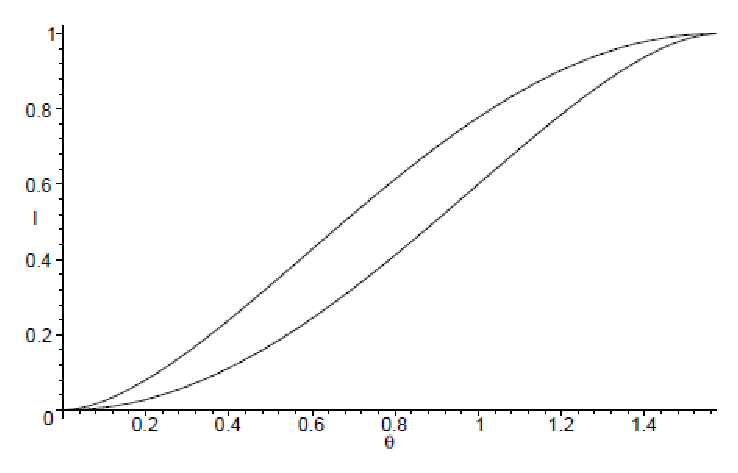
\includegraphics[width=0.5\textwidth]{accessible_information.eps}
            \caption{The von Neumann entropy compared to the accessible information for the ensemble of two quantum states occurring with equal probabilities and differing by an angle of $\theta$, $0 \leq \theta \leq \frac{\pi}{2}$. The top curve is the von Neumann entropy. \cite{shor} \label{fig:accessible}}
    \end{figure}
    which has eigenvalues $\frac{1}{2} \pm \cos\theta$, so the von Neumann entropy of the density matrix is $S(\rho) = H \left( \frac{1}{2} - \frac{\cos\theta}{2} \right)$. The values of $I_{\text{acc}}$ and $S$ are plotted in Figure \ref{fig:accessible}; it can be observed that $S \geq I_{\text{acc}}$. \par
    In fact, the upper bound
    \begin{align}
        I_{\text{acc}}(\mathcal{E}) \leq S(\rho)
    \end{align}
    holds in general, and we have seen that the equality condition is met in the classical case where $S(\rho) = H(X)$, and $I(X; Y) \leq H(X)$ from classical information theory. For nonorthogonal states, however, $S(\rho) < H(X)$ so that the above is a stronger statement.
    An even stronger statement can be obtained if we consider the accessible information per letter in a message containing $n$ letters. Now, Bob has the choice to perform a measurement on all $n$ letters simultaneously, allowing him to obtain more information than if he were required to measure the letters one at a time. In addition, Alice has the ability to prepare an ensemble of deterministic messages that maximizes distinguishability, rather than constructing messages by selecting letters randomly from the ensemble $\mathcal{E}$. \par
    Alice and Bob can then deduce a code such that the marginal ensemble for each letter is $\mathcal{E}$, and the accessible information for each letter approaches $S(\rho)$ in the limit as $n \to \infty$, so $S(\rho)$ characterizes the accessible information of an ensemble of pure quantum states. The generalization to mixed quantum states is given by the following theorem.
    \begin{theorem}[Holevo]
        Suppose we have a source $\mathcal{E}$ that emits state $\rho_x$ (possibly a mixed state) with probability $p_x$. Then
        \begin{align}
            I_{\textnormal{acc}}(\mathcal{E}) \leq \chi(\mathcal{E})
        \end{align}
        with equality if and only if all the $\rho_x$ commute and are hence simultaneously diagonalizable.
    \end{theorem}
    The equality condition is met in the classical case as expected, and when $\rho_i$ are mutually orthogonal mixed states. Furthermore, if Alice and Bob choose an $n$-letter code where the marginal ensemble for each letter is $\mathcal{E}$ and all code words are required to be \textit{product} states, and Bob performs an optimal POVM on all $n$ letters collectively, then the optimal obtainable accessible information per letter is $\chi(\mathcal{E})$. \par
    An alphabet of mixed quantum states might arise if Alice sends pure quantum states to Bob through a noisy quantum channel and hence the system experiences decoherence. Here, $\chi(\mathcal{E})$ characterizes the maximal amount of classical information that can be trasmitted to Bob if he decodes the mixed states. The states might be those of photons that are initially unentangled. If the noise acts on each photon independently, then $\chi(\mathcal{E})$ is the maximal amount of information given by one photon, and since
    \begin{align}
        \chi(\mathcal{E}) \leq S(\rho) \leq 1,
    \end{align}
    an unentangled photon can carry at most one bit of classical information.

    \subsection{Proof of the Holevo Bound}
    The Holevo bound is easily established if we assume the strong subadditivity property of von Neumann entropy. Recall the scenario in which Alice prepares a quantum state drawn from the ensemble $\mathcal{E} = \{ rho_x, p_x \}$ and Bob follows by performing the POVM $\{ F_y \}$. The joint probability of the preparation $x$ and measurement outcome $y$ is
    \begin{align}
        \mathbb{P}(X = x, Y = y) = p_x \text{Tr} \{ F_y \rho_x \},
    \end{align}
    and we want to show that
    \begin{align}
        I(X; Y) \leq \chi(\mathcal{E}).
    \end{align}
    Recall that strong subadditivity is a property of three subsystems. In addition to the quantum system $Q$ we will prepare an additional input system $X$ that stores a classical record of which preparation was chosen and an output system $Y$ whose classical correlations with $x$ are determined by the joint probability distribution $\mathbb{P}(X = x, Y = y)$. Suppose that the initial state of the combined system $XQY$ is
    \begin{align}
        \rho_{XQY} = \sum_x p_x \dyad{x}{x} \otimes \rho_x \otimes \dyad{0}{0}
    \end{align}
    where the $\ket{x}$s are mutually orthogonal pure states of $X$, and $\ket{0}$ is a particular pure state of $Y$. Performing partial traces gives the results
    \begin{align}
        \rho_X &= \sum_x p_x \dyad{x}{x} \to S(\rho_X) = H(X) \\
        \rho_Q &= \sum_x p_x \rho_x \equiv \rho \to S(\rho_{QY}) = S(\rho_Q) = S(\rho),
    \end{align}
    From the mutual orthogonality of the pure states, we also have
    \begin{align}
        S(\rho_{XQY}) &= S(\rho_{XQ}) = \sum_x -\text{Tr}(p_x \rho_x \log p_x \rho_x \\
        &= H(X) + \sum_x p_x S(\rho_x).
    \end{align}
    Now, we will perform a new unitary transformation which can be described as imprinting the measurement result in the output system $Y$. Consider the situation where Bob specifically performs the orthogonal measurement $\{ E_y \}$ where
    \begin{align}
        E_y E_{y'} = \delta_{yy'} E_y. \label{eq:imprint}
    \end{align}
    The unitary transformation $U_{QY}$ acts on $QY$ according to
    \begin{align}
        \ket{\varphi}_Q \otimes \ket{0}_Y \to \sum_y E_y \ket{\varphi}_Q \otimes \ket{y}_Y
    \end{align}
    where the $\ket{y}$s are mutually orthogonal, and hence transforms $\rho_{XQY}$ as
    \begin{align}
        \rho_{XQY} \to \rho'_{XQY} = \sum_{x, y, y'} p_x \dyad{x}{x} \otimes E_y \rho_x E_{y'} \otimes \dyad{y}{y'}. \label{eq:xqy}
    \end{align}
    Recall that von Neumann entropy is invariant under a unitary change of basis, which allows us to say that
    \begin{align}
        S(\rho'_{XQY}) &= S(\rho_{XQY}) = H(x) + \sum_x p_x S(\rho_x) \\
        S(\rho'_{QY}) &= S(\rho_{QY}) = S(\rho),
    \end{align}
    and taking a partial trace of the right-hand side of (\ref{eq:xqy}) and using (\ref{eq:imprint}), we find that
    \begin{align}
        \rho'_{XY} &= \sum_{x, y} p_x \text{Tr}(E_y \rho_x) \dyad{x}{x} \otimes \dyad{y}{y} \\
        &= \sum_{x, y} p(x, y) \dyad{x, y}{x, y} \\
        &\to S(\rho'_{XY}) = H(X, Y).
    \end{align}
    As a result,
    \begin{align}
        \rho'_Y = \sum_y p(y) \dyad{y}{y} \to S(\rho'_Y) = H(Y).
    \end{align}
    At this point, we may invoke strong subaddivity, which gives us
    \begin{gather}
        S(\rho'_{XQY}) + S(\rho'_Y) \leq S(\rho'_{XY}) + S(\rho'_{QY}) \\
        H(X) + \sum_x p_x S(\rho_x) + H(Y) \leq H(X, Y) + S(\rho) \\
        I(X; Y) = H(X) + H(Y) - H(X, Y) \leq S(\rho) - \sum_x p_x S(\rho_x) = \chi(\mathcal{E}),
    \end{gather}
    the Holevo bound. \par
    We can also extend the Holevo bound to more general POVMs by enlarging the system to include one more subsystem $Z$ and constructing a unitary $U_{QYZ}$ which performs the transformation
    \begin{align}
        \ket{\varphi}_Q \otimes \ket{0}_Y \otimes \ket{0}_Z = \sum_y \sqrt{F_y} \ket{\varphi}_A \otimes \ket{y}_Y \otimes \ket{y}_Z
    \end{align}
    so that
    \begin{align}
        \rho'_{XQYZ} = \sum_{x, y, y'} p_x \dyad{x}{x} \otimes \sqrt{F_y} \rho_x \sqrt{F_{y'}} \otimes \dyad{y}{y'} \otimes \dyad{y}{y'}.
    \end{align}
    Taking the partial trace over $Z$,
    \begin{align}
        \rho'_{XQY} = \sum_{x, y} p_x \dyad{x}{x} \otimes \sqrt{F_y} \rho_x \sqrt{F_y} \otimes \dyad{y}{y}
    \end{align}
    and finally,
    \begin{align}
        \rho'_{XY} &= \sum_{x, y} p_x \text{Tr}(F_y \rho_x) \dyad{x}{x} \otimes \dyad{y}{y} \\
        &= \sum_{x, y} p(x, y) \dyad{x, y}{x, y} \\
        &\to S(\rho'_{XY}) = H(X, Y).
    \end{align}
    We can now apply the previous argument to obtain a similar result.

    \subsection{Case Study: The Peres-Wootters Method}
    Consider a one-qubit example in which Alice prepares one of the three possible pure states
    \begin{align}
        \ket{\varphi_1} &= \left( \begin{array}{c}
            1 \\
            0
        \end{array} \right) \\
        \ket{\varphi_2} &= \left( \begin{array}{c}
            -\frac{1}{2} \\
            \frac{\sqrt{3}}{2}
        \end{array} \right) \\
        \ket{\varphi_3} &= \left( \begin{array}{c}
            -\frac{1}{2} \\
            -\frac{\sqrt{3}}{2}
        \end{array} \right),
    \end{align}
    which describes a spin-$\frac{1}{2}$ object that points in one of three directions symmetrically distributed in the $xz$-plane; each state has an \textit{a priori} probability $\frac{1}{3}$. The states are nonorthogonal because
    \begin{align}
        \braket{\varphi_1}{\varphi_2} = \braket{\varphi_1}{\varphi_3} = \braket{\varphi_2}{\varphi_3} = -\frac{1}{2}. \label{eq:inner3}
    \end{align}
    The density matrix of the ensemble is
    \begin{align}
        \rho = \frac{1}{3} \sum_{i = 1}^3 \dyad{\varphi_i}{\varphi_i} = \frac{1}{2} I,
    \end{align}
    and hence $S(\rho) = 1$. From the Holevo bound, the mutual information of the preparation and the measurement outcome cannot exceed 1 bit. \par
    In reality, the accessible information is much less because of the high level of symmetry in the ensemble allows for easier guessing of the optimal measurement. Bob may choose the three-outcome POVM where
    \begin{align}
        F_a = \frac{2}{3}(I - \dyad{\varphi_a}{\varphi_a}), \quad a = 1, 2, 3, \label{eq:povm3}
    \end{align}
    which has
    \begin{align}
        \mathbb{P}(a | b) = \matrixel{\varphi_b}{F_a}{\varphi_b} = \begin{cases}
            0, & a = b \\
            \frac{1}{2}, & a \neq b
        \end{cases}.
    \end{align}
    In other words, the measurement outcome $a$ excludes the possibility that Alice prepared $a$ but leaves $\textit{a posteriori}$ probabilities of $\frac{1}{2}$ for the remaining two states. The information gained by Bob is
    \begin{align}
        I = H(X) - H(X | Y) = \log_2 3 - 1 \approx .58496. \label{eq:mutual3}
    \end{align}
    The optimality of this measurement can be proven using a variation of a theorem by Davies \cite{preskill}. \par
    Now consider the two-qubit example where each qubit is drawn from the same ensemble. Now suppose that Alice prepares one of nine states
    \begin{align}
        \ket{\varphi_a} \ket{\varphi_b}, \quad a, b = 1, 2, 3,
    \end{align}
    each occurring with probability $p_{ab} = \frac{1}{9}$. In this case, then the optimal strategy is for Bob to perform the POVM (\ref{eq:povm3}) on each of the qubits, achieving the same mutual information as that given by (\ref{eq:mutual3}) for each qubit. \par
    However, it is possible that there is a better strategy for Alice to pursue. If she prepares one of three states given by
    \begin{align}
        \ket{\Phi_a} = \ket{\varphi_a} \ket{\varphi_a}, \quad a = 1, 2, 3, \label{better3}
    \end{align}
    each occurring with probability $p_a = \frac{1}{2}$, then the two qubits are now marked by classical correlations. The three states are linearly independent, so they span a three-dimensional subspace of the four-dimensional two-qubit Hilbert space. The density matrix
    \begin{align}
        \rho = \frac{1}{3} \sum_{a = 1}^3 \dyad{\Phi_a}{\Phi_a}
    \end{align}
    has the nonzero eigenvalues $\frac{1}{2}$, $\frac{1}{4}$, $\frac{1}{4}$, and hence
    \begin{align}
        S(\rho) = -\frac{1}{2} \log \frac{1}{2} - 2 \left( \frac{1}{4} \log \frac{1}{4} \right) = \frac{3}{2}.
    \end{align}
    According to the Holevo bound, the accessible information per qubit is less than $\frac{3}{4}$ bit. This gives the possibility that the mutual information might exceed that given in (\ref{eq:mutual3}) for each qubit. Although the number of signals is fewer, the signals are also more distinguishable, as
    \begin{align}
        \braket{\Phi_a}{\Phi_b} = \frac{1}{4}, \quad a \neq b
    \end{align}
    in contrast to (\ref{eq:inner3}). Due to this higher distinguishability, performing collective instead of separate measurements on the two qubits will provide Bob with a better result. The optimal measurement is no longer obvious, but the following general procedure produces a POVM called the \textit{pretty good measurement} (\textit{PGM}) that is close to optimal. \par
    Consider a collection of vectors $\ket*{\tilde{\Phi}_a}$ that are not necessarily orthogonal or normalized. The goal is to find a POVM that can best distinguish these vectors. Begin by letting 
    \begin{align}
        G = \sum_a \dyad*{\tilde{\Phi}_a}{\tilde{\Phi}_a}.
    \end{align}
    $G$ is a positive operator on the space spanned by the vectors, and hence has an inverse $G^{-1}$ with a positive square root $G^{-1/2}$. Following this, define
    \begin{align}
        F_a = G^{-1/2} \dyad*{\tilde{\Phi}_a}{\tilde{\Phi}_a} G^{-1/2}.
    \end{align}
    We see that
    \begin{align}
        \sum_a F_a &= G^{-1/2} \left( \sum_a F_a \dyad*{\tilde{\Phi}_a}{\tilde{\Phi}_a} \right) G^{-1/2} \\
        &= G^{-1/2} G G^{-1/2} = I
    \end{align}
    on the span of the vectors. The $F_a$'s can be augmented by an additional positive operator, the projection $F_0$ onto the span's orthogonal complement to construct a POVM, which is the PGM associated with the vectors $\ket*{\tilde{\Phi}_a}$. \par
    In the case where the $\ket*{\tilde{\Phi}_a}$'s are orthogonal,
    \begin{align}
        \ket*{\tilde{\Phi}_a} = \sqrt{\lambda_a} \ket{\Phi_a}
    \end{align}
    where the $\sqrt{\lambda_a} \ket{\Phi_a}$ are orthonormal, and we have
    \begin{align}
        F_a &= \sum_{a, b, c}(\ket{\Phi_b} \lambda_b^{-1/2} \bra{\Phi_b})(\lambda_a \dyad{\Phi_a}{\Phi_a})(\ket{\Phi_c} \lambda_c^{-1/2} \bra{\Phi_c}) \\
        &= \dyad{\Phi_a}{\Phi_a}
    \end{align}
    which is the orthogonal measurement that perfectly distinguishes the $\ket{\Phi_a}$ and so is clearly optimal. If the $\ket*{\tilde{\Phi}_a}$ are linearly independent but not orthogonal, then the PGM is again an orthogonal measurement due to the requirements for a POVM, but the measurement is no longer necessarily optimal. \par
    After constructing a PGM for the $\ket{\Phi_a}$'s in (\ref{better3}), we have that
    \begin{align}
        \mathbb{P}(a | a) &= \matrixel{\Phi_a}{F_a}{\Phi_a} = \frac{1}{3} \left( 1 + \frac{1}{\sqrt{2}} \right)^2 \approx .971405 \\
        \mathbb{P}(b | a) &= \matrixel{\Phi_b}{F_b}{\Phi_a} = \frac{1}{6} \left( 1 - \frac{1}{\sqrt{2}} \right)^2 \approx .0142977
    \end{align}
    whenever $b \neq a$. Then it follows that the conditional entropy of the input is
    \begin{align}
        H(X | Y) \approx .215893
    \end{align}
    and since $H(X) = \log_2 3 \approx 1.58496$, the information gain is
    \begin{align}
        I = H(X) - H(X | Y) \approx 1.36907,
    \end{align}
    or a mutual information of about .684535 bits per qubit. Although the Holevo bound is $I < 1.5$ in this case, this result is better than that for a single qubit. \par
    This example was first developed by Peres and Wootters and in summary tells us that distinguishability takes precedence over the number of possible signals for better encoding, and that collective measurement projecting the signal onto a basis of entangled states provides better information retrieval than measuring each qubit separately. Furthermore, although not necessarily optimal, the PGM provides the most information gain of any measurement known so far.

    \subsection{Attaining the Holevo Bound in Pure States}
    Given an ensemble of pure states, our goals is to construct $n$-letter codewords that asymptotically attain an accessible information of $S(\rho)$ per letter. In other words, Alice can choose $2^{n(S - \delta)}$ codewords such that Bob can determine which one was sent, with a negligible probability of error as $n \to \infty$. \par
    In random coding, Alice chooses product signal states
    \begin{align}
        \ket{\varphi_{x_1}} \ket{\varphi_{x_2}} \cdots \ket{\varphi_{x_n}}
    \end{align}
    by drawing each letter at random from the ensemble $\mathcal{E} = \{ \ket{\varphi_x}, p_x \}$. For a typical code, each typical codeword has a large overlap with a typical subspace $\Lambda^{(n)}$ with $\dim \Lambda^{(n)} > 2^{n(S(\rho) - \delta)}$, and the marginal ensemble from which each letter is selected is close to $\mathcal{E}$. The typical subspace is very large for large $n$, which means that Alice can choose a high number of codewords while the typical overlap of two typical codewords remains small. The typical codewords are randomly distributed in the typical subspace, and two randomly chosen unit vectors in a space of dimension $D$ have an average overlap of $\frac{1}{D}$. Thus, if $\ket{u}$ and $\ket{w}$ are two codewords, then
    \begin{align}
        \langle|\langle u | w \rangle|^2\rangle_\Lambda < 2^{-n(S - \delta)}
    \end{align}
    where $\langle \cdot \rangle_\Lambda$ denotes an average over random typical codewords. \par
    The typical codewords are indeed uniformly distributed in the typical subspace, because when averaged over the ensemble, the overlap of random codewords $\ket{\varphi_{x_1}} \cdots \ket{\varphi_{x_n}}$ and $\ket{\varphi_{y_1}} \cdots \ket{\varphi_{y_n}}$ is
    \begin{align}
        \sum p_{x_1} \cdots p_{x_n} p_{y_1} \cdots p_{y_n} \left( |\langle \varphi_{x_1} | \varphi_{y_1} \rangle|^2 \cdots |\langle \varphi_{x_n} | \varphi_{y_n} \rangle|^2 \right) = \text{Tr}(\rho \otimes \cdots \otimes \rho)^2.
    \end{align}
    Now suppose that the trace is restricted to the typical subspace $\Lambda^{(n)}$, which has $\dim \Lambda^{(n)} < 2^{n(S + \delta)}$. The eigenvalues of $\rho^{(n)} = \rho \otimes \cdots \otimes \rho$ restricted to $\Lambda^{(n)}$ satisfy $\lambda < 2^{{-n}(S - \delta)}$. Therefore,
    \begin{align}
        \langle|\langle u | w \rangle|^2\rangle = \text{Tr}_\Lambda \left[ \rho^{(n)} \right]^2 < 2^{n(S + \delta)} \left[ 2^{{-n}(S - \delta)} \right]^2 = 2^{{-n}(S - 3\delta)}
    \end{align}
    where the trace is taken in the typical subspace $\Lambda$. \par
    Also, suppose that $2^{(S - \delta)}$ random codewords $\{ \ket{u_i} \}$ are selected. Then if $\ket{u_j}$ is any fixed codeword,
    \begin{align}
        \sum_{i \neq j} \langle|\langle u_i | u_j \rangle|^2\rangle < 2^{n(S - \delta)} 2^{-n(S - \delta')} + \varepsilon = 2^{-n(\delta - \delta')} + \varepsilon. \label{eq:codewordavg}
    \end{align}
    The sum is taken over all the codewords, and the average is no longer restricted to the typical codewords, which accounts for the $\varepsilon$ on the right-hand side. Given any $\delta$, we may choose $\delta'$ and $\varepsilon$ to be arbitrarily small for $n$ sufficiently large, and hence the codewords become highly distinguishable as $n \to \infty$. \par
    Because (\ref{eq:codewordavg}) holds when we average over codes, it also holds when we average over the particular codeword $\ket{u_j}$. Discarding at most half of the codewords ensures that the codewords are all highly distinguishable from one another. \par
    Alice can choose $2^{n(S - \delta)}$ highly distinguishable codewords, which become mutually orthogonal as $n \to \infty$, and Bob can perform a measurement which is a PGM at finite $n$ but approaches an optimal orthogonal measurement as $n \to \infty$. Then the accessible information per letter
    \begin{align}
        \frac{1}{n} I_\text{acc} \left( \tilde{\mathcal{E}}^{(n)} \right) = S(\rho) - \delta
    \end{align}
    is attainable, where $\tilde{\mathcal{E}}^{(n)}$ denotes the ensemble of $n$-letter codewords. The bound for the probability of error of the POVM has been proved as well \cite{preskill}. \par
    From the Holevo bound and the subadditivity of the von Neumann entropy, the accessible information per letter cannot exceed $S(\rho)$ asymptotically. From the Holevo bound,
    \begin{align}
        I_\text{acc} \left( \tilde{\mathcal{E}}^{(n)} \right) \leq S \left( \tilde{\rho}^{(n)} \right),
    \end{align}
    where $\tilde{\rho}^{(n)}$ denotes the density matrix of the codewords, and from subadditivity,
    \begin{align}
        S \left( \tilde{\rho}^{(n)} \right) \leq \sum_{i = 1}^n S(\tilde{\rho}_i)
    \end{align}
    where $\tilde{\rho}_i$ is the reduced density matrix of the $i$th letter. Since each $\tilde{\rho}_i$ approaches $\rho$ asymptotically, we have that
    \begin{align}
        \lim_{n \to \infty} \frac{1}{n} I_\text{acc} \left( \tilde{\mathcal{E}}^{(n)} \right) \leq \lim_{n \to \infty} \frac{1}{n} S \left( \tilde{\rho}^{(n)} \right) \leq S(\rho)
    \end{align}
    This shows that $S(\rho)$ is asymptotically the optimal accessible information per letter, and this bound applies even if the codewords are entangled states rather than product states. \par
    We can now define the \textit{fixed-alphabet capacity}, or the channel capacity for an alphabet of pure quantum states. Suppose that Alice can choose the \textit{a priori} probabilities of a specific set of quantum states $\ket{\varphi_x}$. Then the fixed-alphabet capacity $C_{f_a}$ is the maximum accessible information over all possible distributions $\{ p_x \}$, and is given by
    \begin{align}
        C_{f_a} = \max_{p_x} S(\rho).
    \end{align}
    $C_{f_a}$ is also asymptotically the optimal number of classical bits that can be encoded per letter.

    \subsection{Attaining the Holevo Bound in Mixed States}
    Extending the previous reasoning to the more general situation in which the ensemble contains mixed quantum states. It turns out that it is possible to convey $\chi(\mathcal{E})$ bits of classical information per letter. The reasoning showing that this is true is similar to that in the previous section, beginning with the random coding argument. \par
    Suppose that Alice selects mixed-state codewords, with each letter drawn from the ensemble $\mathcal{E}$. Then each codeword
    \begin{align}
        \rho_{x_1} \otimes \rho_{x_2} \otimes \cdots \otimes \rho_{x_n}
    \end{align}
    is chosen with probability $p_{x_1} p_{x_2} \cdots p_{x_n}$. In a sense, each typical codeword can now be regarded as an ensemble of pure states, with nearly all of its support on a certain typical subspace. If we average over the codewords, the mean entropy of each codeword is
    \begin{align}
        \langle S^{(n)} \rangle = \sum_{x_1 \cdots x_n} p_{x_1} p_{x_2} \cdots p_{x_n} S(\rho_{x_1} \otimes \rho_{x_2} \otimes \cdots \otimes \rho_{x_n}).
    \end{align}
    Using additivity of entropy of product states and the probability postulate that $\sum_x p_x = 1$, we have that
    \begin{align}
        \langle S^{(n)} \rangle = n \sum_x p_x S(\rho_x) \equiv n \langle S \rangle.
    \end{align}
    For large $n$, the entropy of a codeword $\rho_{x_1} \otimes \rho_{x_2} \otimes \cdots \otimes \rho_{x_n}$ is close to this mean and the eigenvalues of $\rho_{x_1} \otimes \rho_{x_2} \otimes \cdots \otimes \rho_{x_n}$ are close to $2^{-n \langle S \rangle}$. This means that the typical codeword has its support on a typical subspace of dimension $2^{n \langle S \rangle}$. This is analogous to the observation used to prove Shannon's noisy channel coding theorem that the number of typical messages received when a typical message is sent through a noisy classical channel is $2^{nH(Y | X)}$. \par
    For each typical message $x_1 x_2 \cdots x_n$, Bob can construct a \textit{decoding subspace} of dimension $2^{n(\langle S \rangle + \delta)}$, such that the message has a low probability of having nearly all its support on this subspace. He can then also construct a POVM that determines in which decoding subspace the message lies; if the decoding subspaces have little overlap, then errors in decoding are unlikely. \par
    Suppose that Bob performs the PGM determined by all the vectors that span all the typical subspaces in Alice's codewords. If the number of codewords is not too large, this PGM will approach an orthogonal measurement for large $n$. Then the result is likely to be contained in the typical subspace of dimension $2^{n S(\rho)}$ determined by the source $\rho \otimes \rho \otimes \cdots \rho$, as well as in the decoding subspace of the message that Alice sent. Because the measurement results are uniformly distributed in a space of dimension $2^{nS}$ and the pure-state ensemble determined by a particular decoding subspace has dimension $2^{n(\langle S \rangle + \delta)}$, the average overlap of the vector determined by Bob's result with a typical decoding subspace is
    \begin{align}
        \frac{2^{nS}}{2^{n(\langle S \rangle + \delta)}} = 2^{-n(S - \langle S \rangle - \delta)} = 2^{-n(\chi - \delta)}.
    \end{align}
    If Alice chooses $2^{nR}$ codewords, then the average probability of a decoding error is
    \begin{align}
        2^{nR} 2^{-n(\chi - \delta)} = 2^{-n(\chi - R - \delta)}.
    \end{align}
    If $R$ is any number smaller than $\chi$, then the probability of error approaches zero as $n \to \infty$. \par
    As before, we can choose a particular typical code, and discard codewords to achieve a small probability of error for every codeword, so that the marginal ensemble for each codeword approaches $\mathcal{E}$ as $n \to \infty$. In conclusion, it is possible to attain an accessible information of $\chi$ per letter. \par
    The argument bears resemblance to that of the proof of the classical noisy coding theorem; for example, the quantity $\chi$ in the former plays an analogous role to $I$ in the latter.

    \subsection{Classical Capacity of a Quantum Channel}
    When the ensemble consists of three or more states, \textit{block coding} may give a better information transmission rate than $I_\text{acc}$. For example, in a three-state ensemble, using the length-two codewords given by $v_1 \otimes v_1$, $v_2 \otimes v_2$, and $v_3 \otimes v_3$ may use a number of bits that is less than $I_\text{acc}$. As the length of the codewords increases, the information transmission rate improves up to a certain limit, which is given by the following theorem.
    \begin{theorem}[Holevo, Schumacher-Westmoreland]
        The classical capacity obtainable using codewords composed of signal states $\rho_i$, each with probability $p_i$, is
        \begin{align}
            \chi = S \left( \sum_i p_i \rho_i \right) - \sum_i p_i S(\rho_i). \label{eq:capacity}
        \end{align}
    \end{theorem}
    The proof of the theorem in the special case where the $\rho_i$ are pure states uses random codes, typical subspaces, and the square root measurement (also called the ``pretty good measurement'') and is given as follows. Suppose that we are attempting to distinguish between vectors $u_1, u_2, \cdots, u_n$ which appear with equal probability, and let $\phi = \sum_i v_i v_i^\dagger$. The square root measurement is given by the elements
    \begin{align}
        E_i = \phi^{-1/2} v_i v_i^\dagger \phi^{-1/2},
    \end{align}
    which form a POVM because
    \begin{align}
        \sum_i E_i = \phi^{-1/2} \left( \sum_i v_i v_i^\dagger \right) \phi^{-1/2} = I.
    \end{align}
    If we choose $N$ codewords $u_j = v_{i_1} \otimes v_{i_2} \otimes \cdots \otimes v_{i_n}$, where the $v_i$ are chosen at random with probability $p_i$, then we can use the codewords $u_j$ to send information that can be identified with high probability. The decoding process consists of the following steps:
    \begin{enumerate}
        \item
            Project into the typical subspace $\mathcal{T}$. This projection is successful with high probability, giving the result $\tilde{u}_j = P_\mathcal{T} u_j$ where $P_\mathcal{T}$ is the projection matrix on to the subspace $\mathcal{T}$.

        \item
            Perform the square root measurement on the $\tilde{u}_j$.
    \end{enumerate}
    The probability of error is given by
    \begin{align}
        1 - \frac{1}{N} \sum_{j = 1}^N |\tilde{u}_j \phi^{-1/2} \tilde{u}_j|^2.
    \end{align}
    Although the proof will be omitted, an intuition for why this procedure is correct is that for the probability of error to be small, $\phi^{-1/2} \tilde{u}_j$ must be close to $\tilde{u}_j$ for most $j$. One way to see why $\phi^{-1/2} \tilde{u}_j$ is close to $\tilde{u}_j$ is because the $\tilde{u}_j$ are distributed more or less randomly in the typical subspace $\mathcal{T}$, so $\phi = \sum_j \tilde{u}_j \tilde{u}_j^\dagger$ is close to the identity matrix on its support. By the Holevo bound, a $d$-dimensional quantum state space can hold at most $d$ bits of information, which means that being able to distinguish the $\tilde{u}_j$ requires that $N < \text{dim} \mathcal{T}$. \par
    Unlike the classical capacity, the capacity of a quantum channel does not yet have a known formula. A good starting point for the capacity of a quantum channel $\mathcal{N}$ is the maximum of $\chi$ over all possible distributions of channel outputs, or
    \begin{align}
        \chi_{\text{max}}(\mathcal{N}) = \max_i \chi \bigl( \{(\mathcal{N}(\rho_i), p_i)\} \bigr),
    \end{align}
    because the sender can communicate any of the states $\mathcal{N}(\rho_i)$ to the receiver. However, it is possible that the capacity may be further increased by properties such as entanglement between the separate inputs to the channel. One way to restate the problem is to ask whether $\chi_\text{max}$ is \textit{additive}, or
    \begin{align}
        \chi_\text{max}(\mathcal{N}_1 \otimes \mathcal{N}_2) = \chi_\text{max}(\mathcal{N}_1) + \chi_\text{max}(\mathcal{N}_1)
    \end{align}
    for two quantum channels $\mathcal{N}_1$ and $\mathcal{N}_2$. Note that it is easy to prove $\textit{subadditivity}$ of this quantity, but strict additivity can be proved, then it will show that using the tensor product of two channels jointly allows for a strictly higher capacity.


    \section{Quantifying Entanglement}
    The results known as quantum teleportation and superdense coding can also be considered as part of quantum information theory. Teleportation can be used to send qubits over a classical channel if both the sender and the receiver possess \textit{shared EPR pairs} (a form of entanglement), which leads to the question of how many EPR pairs can be shared when the two parties use only classical communication but can perform quantum operations on their own local states. \par
    Let the two parties' quantum state spaces be $A$ and $B$, and $\rho \in A \otimes B$ be a pure state. Then $n$ copies of $\rho$ can be used to produce
    \begin{align}
        n S(\text{Tr}_A \rho) + o(n) = n S(\text{Tr}_B \rho) + o(n)
    \end{align}
    nearly perfect EPR pairs and vice versa, where the fidelity between the actual and desired states approaches $1$ as the block length $n$ goes to infinity. \par
    If $\rho$ is not a pure state, then the answer to the problem of quantifying entanglement is no longer known, but we can start by defining the following.
    \begin{definition}
        Suppose that $\rho_{AB}$ is a mixed state shared by Alice and Bob, who each possess $n$ identical copies of this state, and that they can prepare $(\rho_{AB})^n$ with asymptotically high fidelity and probability of success from $k$ EPR pairs using only classical communication and local quantum operations. Then the \textit{entanglement of formation} $E_F$ of $\rho_{AB}$ is given by
        \begin{align}
            E_F(\rho_{AB}) = \lim_{n \to \infty} \frac{k_\text{min}}{n}.
        \end{align}
        Furthermore, suppose that Alice and Bob can distill $k'$ EPR pairs from $n$ copies of $\rho_{AB}$ using only classical communication and local operations. Then the \textit{entanglement of distillation} $E_D$ of $\rho_{AB}$ is given by
        \begin{align}
            E_D(\rho_{AB}) = \lim_{n \to \infty} \frac{k'_\text{max}}{n}.
        \end{align}
    \end{definition}
    In other words, these definitions characterize asymptotically the number of EPR pairs that are needed to form $\rho$ and the number of EPR pairs that can be created from $\rho$, respectively. $E_F$ and $E_D$ were clearly equal in the previous case where $\rho$ was a pure state, but in the mixed case, no explicit formulas are known. Since entanglement cannot be created locally, we do know that $E_D \leq E_F$. \par
    Furthermore, it is conjectured that the inequality is strict, because preparing the mixed state $(\rho_{AB})^n$ from the pure state $(\ket{\phi^+}_{AB} \leftidx{_{AB}^{}}{\bra{\phi^+}}{_{}^{}})^k$ requires the discarding of quantum information. The \textit{one-shot entanglement of formation}
    \begin{align}
        E_{F, 1}(\rho) = \min_{\sum_i p_i \rho_i = \rho} \sum_i p_i S(\text{Tr}_A \rho_i),
    \end{align}
    which is the minimum average entanglement over ensembles of pure states whose density matrix is $\rho$, provides a possible expression for the entanglement of formation, but only if it can be proved to be additive \cite{shor}. \par
    We can further distinguish different types of entanglement of distillation based on whether classical communication is restricted to one direction or unrestricted. Specifically, we let $E_{D_1}$ denote the number of $EPR$ pairs that can be distilled if only one-way communication is allowed. It is known that $E_{D_1} < E_D$ and hence $E_{D_1} < E_F$ for some mixed states, while $E_{D_1} = E_D = E_F$ for pure states. \par
    Mixed-state entanglement, especially when communication is restricted to one direction, is related to the transmission of quantum information through noisy quantum channels. If the noise of a quantum channel described by a superoperator $\$$ is within a certain threshold, then we can construct an $n$-letter block code such that quantum information can pass through the process of encoding, sending through the channel $(\$)^n$, decoding, and recovery with arbitrarily good fidelity as $n \to \infty$. We call the optimal number of encoded qubits per letter than can be transmitted the \textit{quantum channel capacity} $C(\$)$, and it turns out that this quantity is related to $D_1$ of a particular mixed state associated with the channel \cite{preskill}.

    \subsection{Entanglement-Assisted Capacity}
    There is another capacity for quantum channels with a formula that can be proven. Recall that if we have a noiseless quantum channel $\mathcal{N}$ and if the sender and receiver possess shared EPR pairs, then they can use superdense coding to double the classical capacity of $\mathcal{N}$. If $\mathcal{N}$ is noisy, then using shared EPR pairs can still increase the classical capacity to a smaller degree. The \textit{entanglement-assisted capacity} $C_E$ is defined as the quantity of classical information that can asymptotically be sent per channel use if the quantity of shared entanglement is sufficiently high, and is given by the following formula. \cite{shor}
    \begin{theorem}[Bennett, Shor, Smolin Thapliyal]
        The entanglement-assisted capacity is given by
        \begin{align}
            C_E(\mathcal{N}) = \max_{\rho \in \mathcal{H} \otimes \mathcal{S}} S(\textnormal{Tr}_\mathcal{R}(\mathcal{N} \otimes \mathcal{I}) \rho) + S(\textnormal{Tr}_\mathcal{S}(\mathcal{N} \otimes \mathcal{I}) \rho) - S((\mathcal{N} \otimes \mathcal{I}) \rho) \label{eq:assisted}
        \end{align}
        where $\mathcal{R}$ and $\mathcal{S}$ stand for receiver and sender respectively, and $\rho$ is maximized over pure states on the tensor product of the input state space $\mathcal{H} = \mathbb{C}^d$ of the channel and a $d$-dimensional quantum space $\mathcal{S}$ kept by the sender.
    \end{theorem}
    The quantity being maximized is a generalization of mutual information and is called \textit{quantum mutual information}. \par
    The entanglement-assisted capacity relates to a number of applications. In the problem of sending quantum states over a noisy quantum channel, many of the classical capacity theorems are no longer true. The quantum channel capacity is increased by a back channel from the receiver to the sender, which leads to two capacities $Q_2$ and $Q \leq Q_2$ where only $Q_2$ has a back channel. The conjectured capacity formula for $Q$ is similar to the last two terms of (\ref{eq:assisted}) and is given by
    \begin{align}
        Q(\mathcal{N}) = \lim_{n \to \infty} \max_{\rho \in (\mathcal{H} \otimes \mathcal{S})^n} S(\textnormal{Tr}_\mathcal{S}(\mathcal{N} \otimes \mathcal{I}) \rho) - S((\mathcal{N} \otimes \mathcal{I}) \rho)
    \end{align}
    where $\rho$, $\mathcal{H}$, and $\mathcal{S}$ are defined as before. Here, the quantity being maximized is called the \textit{coherent information}. Unlike the classical or the quantum mutual information, the coherent information is not additive, which means that now we must take the maximum over the tensor product of $n$ uses of the channel where $n$ goes to infinity. $Q(\mathcal{N})$ is an upper bound for, and is conjectured to be equal to, the quantum capacity of a noisy quantum channel $\mathcal{N}$.

    \section{The Entropic Uncertainty Principle}
    In this brief section we will give a restatement of the uncertainty principle of quantum mechanics in terms of Shannon entropy. The Heisenberg uncertainty principle states that for any observables $C$ and $D$, the standard deviations $\Delta(C)$ and $\Delta(D)$ must satisfy the relation
    \begin{align}
        \Delta(C) \Delta(D) \geq \frac{|\bra{\psi}[C, D]\ket{\psi}|}{2}
    \end{align}
    for a quantum system in the state $\ket{\psi}$, where $[\cdot, \cdot]$ denotes the commutator. The spectral decompositions of the observables are given by $C = \sum_c c \dyad{c}{c}$ and $D = \sum_d d \dyad{d}{d}$. $f(C, D) \equiv \max_{c, d} | \langle c | d \rangle |$ is defined as the maximum fidelity between any two eigenvectors of $\ket{c}$ and $\ket{d}$.
    \begin{theorem}
        Suppose the quantum system is prepared in a state $\ket{\psi}$, and let $p(c)$ and $p(d)$ respectively denote the probability distributions associated with measurements of $C$ and $D$, with respective associated entropies $H(C)$ and $H(D)$. Then we have that
        \begin{align}
            H(C) + H(D) \geq 2\log \left( \frac{1}{f(C, D)} \right).
        \end{align}
    \end{theorem}
    The full proof of this theorem is attributed to Deutsch; however, a weaker result
    \begin{align}
        H(C) + H(D) \geq -2\log \left( \frac{1 + f(C, D)}{2} \right).
    \end{align}
    can be proved as follows. First, note that
    \begin{align}
        H(C) + H(D) = -\sum_{cd} p(c) q(d) \log(p(c)q(d)) \label{eq:entropysum}
    \end{align}
    and we want to bound $p(c)q(d) = |\langle c | \psi \rangle \langle \psi | d \rangle|^2$ from above.
    Let $\ket*{\tilde{\psi}}$ be the projection of $\ket{\psi}$ onto the space spanned by $\ket{c}$ and $\ket{d}$, so $\ket*{\tilde{\psi}}$ has norm $\lambda \leq 1$.
    If $\theta$ is the angle between $\ket{d}$ and $\ket{c}$ and $\varphi$ is the angle between $\ket*{\tilde{\psi}}$ and $\ket{d}$ in this space, then it can be seen that $p(c)q(d) = |\langle c | \tilde{\psi} \rangle \langle \tilde{\psi} | d \rangle|^2 = \lambda^2 \cos^2(\theta - \varphi) \cos^2(\varphi)$.
    The maximum is reached when $\lambda = 1$ and $\varphi = \theta / 2$, and the maximum value is
    \begin{align}
        p(c)q(d) = \cos^4(\theta / 2) = \left( \frac{1 + |\langle c | d \rangle|}{2} \right)^2.
    \end{align}
    Combining this with (\ref{eq:entropysum}), we have the result
    \begin{align}
        H(C) + H(D) \geq -2\log \left( \frac{1 + f(C, D)}{2} \right).
    \end{align}

    \section{Conclusion}
    In this paper, we have discussed the following topics and results within and related to the field of quantum information theory: \par
    The \textit{Shannon entropy} of an ensemble $X = \{ x, p(x) \}$, given by $H(X) \equiv \langle -\log p(x) \rangle$, quantifies the compressibility of classical information. A message $n$ letters long, where each letter is drawn independently from $X$, can be compressed to $H(X)$ bits per letter and still be decoded with negligible error as $n \to \inf$. \par
    The \textit{mutual information} $I(X; Y) = H(X) + H(Y) - H(X, Y)$ quantifies the correlation of ensembles $X$ and $Y$. Learning the value of $y$ also gives an average of $I(X; Y)$ bits of information about $x$. The capacity $C = \max_{\{ p(x) \}}$ of a memoryless noisy classical channel gives the maximum number of bits per letter than can be transmitted through the channel with negligible error probability as $n \to \infty$. \par
    The \textit{von Neumann entropy} of a density matrix $\rho$ is $S(\rho) = -\text{Tr} \rho \log \rho$, and the \textit{Holevo information} of an ensemble $\mathcal{E} = \{ \rho_x, p_x \}$ of quantum states is $\chi(\mathcal{E}) = S(\sum_x p_x \rho_x) - \sum_x p_x S(\rho_x)$. The von Neumann entropy quantifies the compressibility of an ensemble of pure quantum states. A message $n$ letters long, where each letter is drawn independently from the ensemble $\{ \ket{\varphi_x}, p_x \}$, can be compressed to $S(\rho)$ qubits per letter and still be decoded with negligible error as $n \to \infty$. If the letters are drawn from the ensemble $\mathcal{E}$ of mixed quantum states, then it is not possible to compress the message to fewer than $\chi(\mathcal{E})$ qubits per letter and still preserve high fidelity. The properties of Von Neumann entropy are closely related to those that are used to quantify information in thermodynamics and statistical mechanics. \par
    The \textit{accessible information} of an ensemble $\mathcal{E}$ of quantum states is the maximal number of bits of information that can be acquired about the preparation of the state on average using the \textit{optimal measurement}, and cannot exceed the \textit{Holevo information} of the ensemble. An $n$-letter code can be constructed such that the marginal ensemble for each letter is close to $\mathcal{E}$ and the accessible information for each letter is close to $\chi(\mathcal{E})$. The product state capacity of a quantum channel given by superoperator $\$$, given by $C(\$) = \max_\mathcal{E} \chi(\$(\mathcal{E}))$, applies when each codeword is a tensor product of the letter states, and gives the maximum number of classical bits per letter that can be transmitted through the quantum channel with negligible probability of error as $n \to \infty$. \par
    The \textit{entanglement} $E$ of a bipartite pure state $\ket\psi_{AB}$ is $E = S(\rho_A)$, where $\rho_A = \text{Tr}_B(\ket{\psi}_{AB} \leftidx{_{AB}^{}}{\bra{\psi}}{_{}^{}})$. Using only classical communication and local quantum operations, we can prepare $n$ copies of $\ket{\psi}_{AB}$ from $nE$ EPR pairs, and distill $nE$ EPR pairs from $n$ copies of $\ket{\psi}_{AB}$ asymptotically as $n \to \infty$. \par
    Because quantum information theory is a relatively new and burgeoning field, there are still many widely held conjectures that have yet to be proved, especially those related to characterizing the information of ensembles of mixed states. However, as research progresses, we can expect to see many of these open questions solved. Quantum information theory may eventually play a similar role as classical information theory does today, as applications further involve quantum effects to a greater extent.

    \titleformat{\section}{\normalfont\Large\bfseries}{}{0em}{#1}
    \bibliographystyle{acm}
    \bibliography{references}

\end{document}
